\documentclass{resume}

\usepackage{graphicx}
\usepackage{tabularx}
\usepackage{hyperref}
\usepackage{xcolor}

\hypersetup{
    colorlinks=true,
    linkcolor=blue,
    urlcolor=blue,
}

\begin{document}

\fontfamily{ppl}\selectfont

\noindent
\begin{tabularx}{\linewidth}{@{}m{0.8\textwidth} m{0.2\textwidth}@{}}
{
    \Large{\textbf{Jean-Paul Roisin - Web Developer}}
    \newline
    \small{
        \href{mailto:jeanpaul.roisin@protonmail.com}{jeanpaul.roisin@protonmail.com}
        \textbf{ · } 
        {\fontdimen2\font=0.75ex +32 493 18 38 77} 
        \newline
        \textbf{ · } 
        \href{https://www.linkedin.com/in/jp-roisin}{LinkedIn: jp-roisin} 
        \textbf{ · } 
        \href{https://github.com/jp-roisin}{GitHub: jp-roisin} 
        \newline
        Brussels - Belgium
    }
} & 
{
    \hfill
    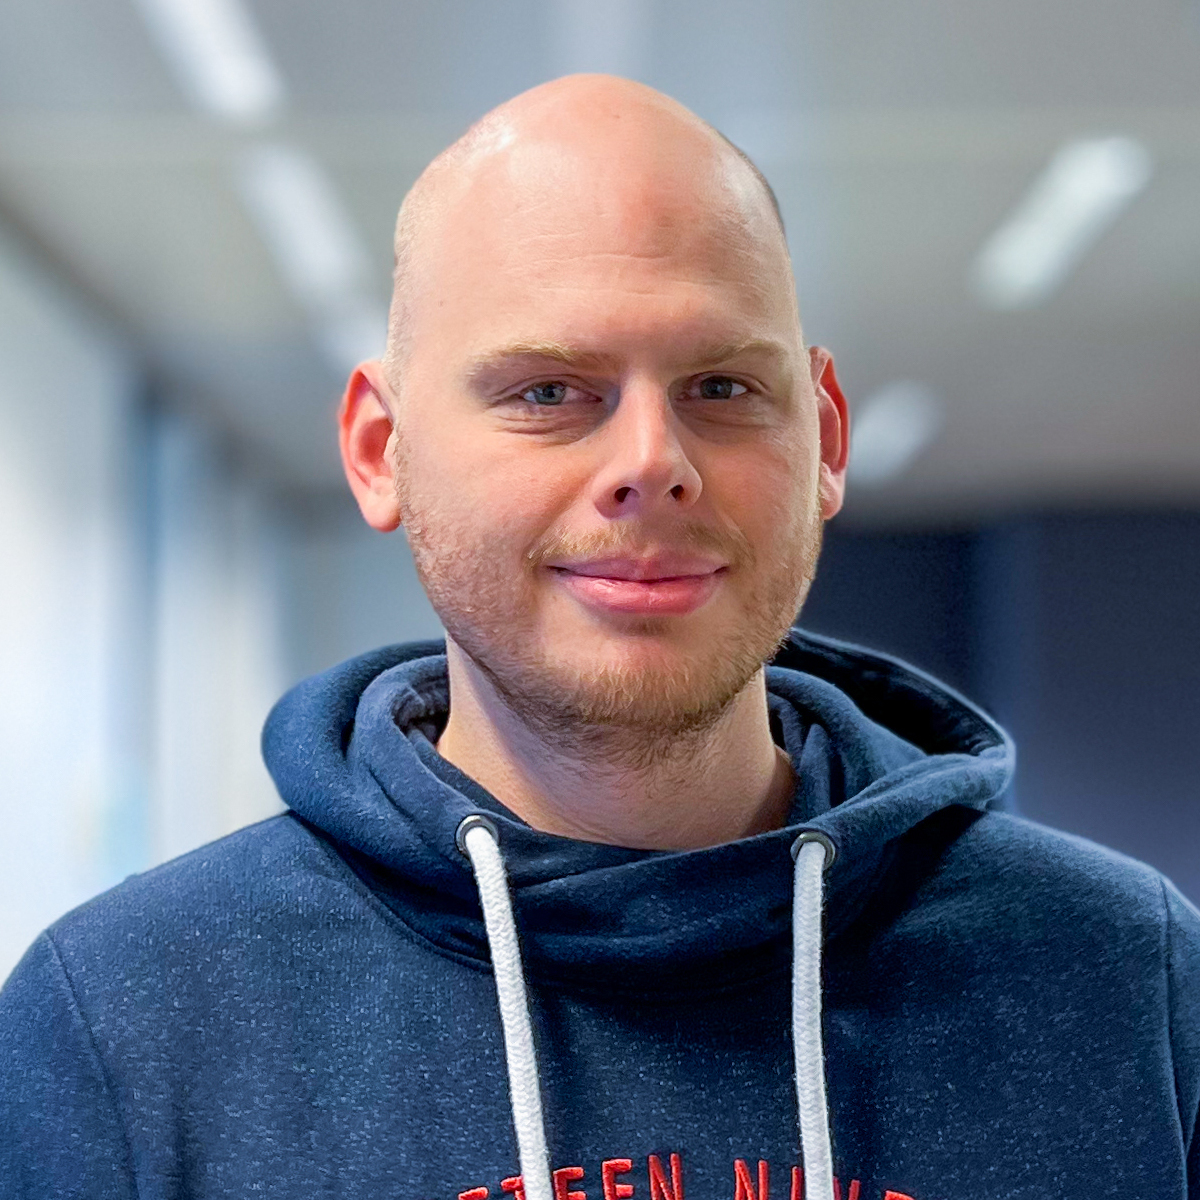
\includegraphics[width=2.8cm]{images/square.jpg}
}
\end{tabularx}
\begin{center}
\begin{tabularx}{\linewidth}{@{}*{2}{X}@{}}
% left side %
{
    \csection{Professional Experience}{\small
        \begin{itemize}
            \item \frcontent{AppTweak}{Frontend development full-time - Brussels}{
              Full-time Frontend Developer in an agile team, contributing to a complex data-driven web app with modern technologies. 
              Proficient in continuous development with a focus on code quality, consistently creating thorough tests for resilient applications.
              Actively engaged in code review and pair coding sessions. 
              Organized and participated in workshops, fostering collaborative learning within the team.
              Took ownership of product features and code segments, ensuring accountability throughout the development process.
              }
              {Nov 2022 - Present}
            \item \frcontent{Igloo}{Web development internship - Louvain-la-Neuve}{
              Full-time intern, actively involved in adding features to a spa.
              Expertise in Next.js, Prisma, and TypeScript.
              Regular daily code reviews with the tech leader to maintain high-quality code standards.
              }
              {Feb 2022 - Jun 2022}
            \item \frcontent{Interparking}{Web development internship - Remote}{
              Interned on the development team overseeing a web and mobile app project.
              Gained insights into the challenges inherent in both web and mobile platforms.
              Thrived in a fully remote, multi-nationality work environment, adapting to diverse collaboration dynamics.
              }
            {Apr 2021 - Jun 2021}
        \end{itemize}
    }
    \csection{Student Jobs}{\small
        \begin{itemize}
            % item 1 %
            \item \frcontent{Volleyball Coach}{
              Coached for multiple years, managing players of various age groups.
            }{}{2014 - 2023}
            % item 2 %
            \item \frcontent{Bartender at La Clef de Verre}{
              Handling bar and table service.
            }{}{2016 - 2017}
        \end{itemize}
    }
} 
% end left side %
& 
% right side %
{
    \csection{Development Skills}{\small
        \begin{itemize}
            \item \textbf{Languages} \newline
            {\footnotesize TypeScript (JavaScript ES6+), Rust, PHP, HTML5, CSS3, and SQL}{}{}
            \item \textbf{Libraries \& Frameworks} \newline
            {\footnotesize React, React-Native, Redux (RTK and Saga), Expo, Jest, Puppeteer, NodeJs, Express, Tailwind, Sass, and Prisma }
            \item \textbf{Tools} \newline
            {\footnotesize Git, GitHub, Docker, Figma, Concourse CI, Storybook, Vim, Tmux, and Linux}
          \item \textbf{Methodologies \& Practices} \newline
            {\footnotesize Scrum, Kanban, Ci/CD, pair programming, conducting workshops, and code reviews}

        \end{itemize}
    }
    \csection{Languages}{\small
        \begin{itemize}
            \item {\footnotesize French (Native)}
            \item {\footnotesize English (C1)}
        \end{itemize}
    }
    \csection{Soft Skills}{\small
        \begin{itemize}
            \item Autonomous and self-taught
            \item Problem solver
            \item Dynamic
        \end{itemize}
    }
    \csection{Education}{\small
        \begin{itemize}
            % item 1 %
            \item \frcontent{Web Development Night Classes}{IFAPME of Charleroi}{}{2020 - 2022}
            \item \frcontent{Bachelor AESI in Mathematics}{ENCBW in Louvain-la-Neuve}{}{2016 - 2020}
        \end{itemize}
    }
    \csection{Interests}{\small
        \begin{itemize}
            \item Volleyball
            \item Chess
        \end{itemize}
    }
}
\end{tabularx}
\end{center}
\end{document}
